\section{Diskontinuierliche Galerkin Methoden}
F\"ur die Galerkin Methoden wurde folgendes f\"ur die Basen vorausgesetzt:
\begin{itemize}
	\item Lineare Unabh\"angigkeit
	\item Kontinuierlich
	\item Kompakter Tr\"ager
\end{itemize}
Die Idee der Diskontinuierlichen Galerkin Methoden besteht darin, die Voraussetzung der Kontinuit\"at aufzul\"osen:
\begin{itemize}
	\item Unstetige Funktionen k\"onnen behandelt werden
	\item Die Masse Matrizen k\"onnen diagonal sein, was den L\"osungsaufwand stark verringert.
\end{itemize}
Das l\"asst sich dadurch implementieren, dass die Grundideen von FV und FEM kombiniert werden. Man verwendet zun\"achst beliebige, an den Elementr\"andern Unstetige Basisfunktionen $\varphi_p(x-x_i)$.
\par
Das weitere Vorgehen ist zun\"achst identisch zu den FEM. Folglich ergibt sich als schwache Formulierung f\"ur die Kontinuit\"atsgleichung:
\begin{align*}
	R(u_{1;0},u_{1;1},\cdots,u_{N;P};x,t) &= \frac{\partial \overline{u}}{\pet} + \frac{\partial f(\overline{u})}{\pex} \\
	\sum_{j,p}\frac{du_{j,p}}{dt}\delta_{ij}\int_{Ii}dx\varphi_{i;p}\varphi_{j;p} + \int_{Ii}dx\varphi_{i;q}\frac{\partial f(\overline{u})}{\pex} &= 0,~~~\forall i=1,\cdots N,\forall q=0,\cdots P
\end{align*}
Bei Diskontinuierlichen Galerkin Methoden sind die Integrale dabei auf dem Element selbst, also in $Ii$ eingeschr\"ankt, da der Tr\"ager kompakt ist. Die Massematrix ist wie bei den FEM Blockdiagonal mit der Blockgr\"o\ss{}e $(P+1)\times(P+1)$. Die Steifigkeitsmatrix muss allerdings anders betrachtet werden:
\par
\begin{equation*}
	\int_{Ii}dx\varphi_{i;q}\frac{\partial f(\overline{u}}{\pex} = \int_{Ii}dx\frac{\partial}{\pex}(\varphi_{i;q}f(\overline{u}) - \int_{Ii}dxf(\overline{u})\frac{\partial\varphi_{i;q}}{\pex}
\end{equation*}
\par
\vspace{-2em}
\begin{tikzpicture}
	\centering
	\node[anchor=south west,inner sep=0] (Bild) at (0,0){};
	\begin{scope}[x=(Bild.south east),y=(Bild.north west)]
		\draw [ultra thick] [->] (160,0) -- (170,10) node [pos=0,below] {verschwindet nicht!};
	\end{scope}
\end{tikzpicture}
\par
Dadurch muss ein neuer Term f\"ur die numerischen Fl\"usse \"uber den Rand eingef\"uhrt werden:
\par
\begin{equation*}
	\int_{Ii}dx\frac{\partial}{\pex}(\varphi_{i;1}f(\overline{u})) = h_i(\overline{u};x_{i+1/2},t)\varphi_{i;q}(x_{i+1/2}) - h_i(\overline{u};x_{i-1/2},t)\varphi_{i;q}(x_{i-1/2})
\end{equation*}
\par
\vspace{-2.5em}
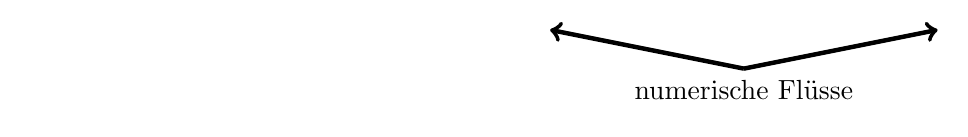
\begin{tikzpicture}
	\centering
	\node[anchor=south west,inner sep=0] (Bild) at (0,0){};
	\begin{scope}[x=(Bild.south east),y=(Bild.north west)]
		\draw [ultra thick] [->] (185,0) -- (135,10) node [pos=0,below] {numerische Fl\"usse};
		\draw [ultra thick] [->] (185,0) -- (235,10) node [pos=0,below] {};
	\end{scope}
\end{tikzpicture}
\par
Die Schwache Formulierung sieht folglich sehr \"ahnlich aus, wie bei FEM, allerdings kommen noch die numerischen Fl\"usse hinzu, welche bei den FEM als Neumann-Randbedingung verschwinden w\"urden.
\par
\begin{equation*}
	\sum_{j,p}\frac{du_{j;p}}{dt}\delta_{ij}\int_{Ii}dx\varphi_{i;q}\varphi_{j;p} - \int_{Ii}dxf(\overline{u})\frac{\partial \varphi_{i;1}}{\pex} + h_i(\overline{u};x_{i+1/2},t)\varphi_{i;q}(x_{i+1/2}) - h_i(\overline{u};x_{i-1/2},t)\varphi_{i;q}(x_{i-1/2}) =  0
\end{equation*}
Im folgenden wird erleutert, wie diese bestimmt werden k\"onnen.

\subsection*{DG numerische Fl\"usse}
Die numerischen Fl\"usse m\"ussen 3 Bedingungen erf\"ullen:
\begin{itemize}
	\item[1] \textbf{Erhaltung}: Fl\"usse sind auf beiden R\"andern des Elements gleich. \\ \hspace*{4em}$h_i(\overline{u},x_{i+1/2},t) = h_{i+1}(\overline{u},x_{i+1/2},t) = h(\overline{u},x_{i+1/2},t)$
	\item[2] \textbf{Lokalit\"at}: Fl\"usse h\"angen nur von der L\"osung rechts und links der Elementgrenze ab. \\
	\hspace*{4em}$h_i(\overline{u},x_{i+1/2},t) = \bs{F}(u^-_{j+1/2}(t), u^+_{j+1/2}(t))$
	\item[3] \textbf{Konsistenz}: Bei Kontinuierlicher Approximation ist der numerische Fluss identisch zum analytischen. \\
	$\bs{F}(u,u) = f(u)$
\end{itemize}

Um Konsistenz zu erhalten sind mehrere Formulierungen f\"ur Fl\"usse m\"oglich. F\"ur den linearen Fall $f(u) = cu$ gilt:
\par
\textbf{1. Der zentrale Fluss}
\begin{equation*}
	\bs{F}(u^-,u^+) = \frac{c}{2}[u^- + u^+]
\end{equation*}
\textbf{2. Upwind Fl\"usse (Godunov oder Lax-Friedrichs}
\begin{equation*}
	\bs{F}(u^-, u^+) = \begin{array}{ll} cu^- ~~~f\"ur ~~~c\geq0 \\ cu^+ ~~~f\"ur ~~~c<0 \end{array}
\end{equation*}
\textbf{3. Allgemeine Schreibweise}
\begin{equation*}
	\bs{F}(u^-,u^+) = c\bigg[ \frac{u^- + u^+}{2} + \alpha(u^- - u^+) \bigg] = c(\{u\} + \alpha[u]) = cu^*
\end{equation*}
Je nachdem wie c und $\alpha$ gew\"ahlt sind, kann die Formulierung angepasst werden. So enth\"alt die Allgemeine Schreibweise auch den zentralen und den upwind Fluss.
Dabei sind die Operatoren wichtig:
\begin{itemize}
	\item \textbf{Mittelwert:} $\{u\}$ 
	\item \textbf{Sprung:} $[u]$
\end{itemize}
Aus der Schwachen Formulierung geht hervor, dass die Massematrix $M^{ij}_{qp} = \delta_{ij}\int_{Ii}dx\varphi_{i;q}\varphi_{j;p}$ Blockdiagonal und damit einfach invertierbar ist. Je nachdem wie die Basisfunktionen gew\"ahlt werden, kann diese sogar komplett diagonal sein.

\subsection*{Basisfunktionen}
\subsubsection*{St\"uckweise konstant:}
\begin{figure*}[ht]
	\centering
	\includegraphics[width=0.5\textwidth]{dgconst}
\end{figure*}
Es folgt f\"ur die L\"osung der Kontinuit\"atsgleichung:
\par
\begin{equation*}
	\dex_i\frac{du_{i+1;0} - u_{i-1;0}}{2} + c\alpha(2u_{i;0} - u{i+1;0} - u_{i-1;0}) = 0
\end{equation*}
Je nach gew\"ahltem c und $\alpha$ ergeben sich die Formen:
\begin{align*}
	1.~\alpha=\frac{1}{2} ~~~&\Rightarrow\frac{du_{i;0}}{dt} + c\frac{u_{i;0} - u_{i-1;0}}{\dex_i} = 0 ~~~ \textrm{upwind} \\
	2.~\alpha = -\frac{1}{2} ~~~&\Rightarrow\frac{du_{i;0}}{dt} + c\frac{u_{i+1;0} - u_{i;0}}{\dex_i} = 0 ~~~ \textrm{downwind} \\
	3.~\alpha = 0 ~~~&\Rightarrow\frac{du_{i;0}}{dt} + c\frac{u_{i+1;0} - u_{i-1;0}}{\dex_i} = 0 ~~~ \textrm{central}
\end{align*}

\subsubsection*{St\"uckweise linear:}
\begin{figure*}[ht]
	\centering
	\includegraphics[width=0.5\textwidth]{dglin}
\end{figure*}
Da die einzelnen Schritte bei DG \"uber Finite Differenzen bestimmt werden, sind die Slopes bereits Bestandteil der Gleichung. Dadurch m\"ussen diese nicht wie bei den FV extra bestimmt werden und Verfahren wie Slope limiters entfallen.

\subsubsection*{Basen h\"oherer Ordnung:}
Der Einfachste Ansatz f\"ur Polynome h\"oherer Ordnung sind die Monomen. Diese stellen die Summe einzelner Polynome dar, bis zu einer definierten Ordnung:
\par
\begin{equation*}
	\varphi_{i;p}(x) \in \{ 1,x-x_i, (x-x_i)^2, \cdots, (x-x_i)^p, x\in[x_{i-1/2}, x_{i+1/2}]  \}
\end{equation*}
Diese ergeben eine Blockdiagonale Massenmatrix, die allerdings mit h\"oherer Ordnung immer st\"arker besetzt ist. Um das zu verhindern eignen sich Orthogonale Basisfunktionen.

\textbf{Legedre Basisfunktionen:}
\begin{multicols}{2}
	\vspace{-2em}
	Die Basen werden folgenderma\ss{}en gew\"ahlt:
	\begin{multline*}
		\varphi_{i;p}(x)\in\bigg{\{} \sqrt{\frac{2p + 1}{\dex_i}} \bs{P}_p\bigg(\frac{x-x_i}{\dex_i/2}\bigg),\cdots \\ \cdots \in[x_{i-1/2}, x_{i+1/2}], p=0,1,\cdots,P \bigg{\}}
	\end{multline*}
	Dadurch ergibt sich f\"ur die Massematrix eine rein diagonale Struktur:
	\begin{equation*}
		M^{ij}_{qp} = \delta_{ij}\int_{Ii}dx\varphi_{i;q}\varphi_{j;p} = \delta_{ij}\delta_{qp}
	\end{equation*}
\vfill\null
\columnbreak
	\includegraphics[width=0.5\textwidth]{legendre}
\end{multicols}

\subsection{Semidiskrete Stabilit\"at}
Durch die Anpassung der Parameter c und $\alpha$ kann auch die Ausbreitung und damit auch die Stabilit\"at beeinflusst werden. Schaut man erneut die Allgemeine Form des Flusses an, so f\"allt auf, dass folgende Bedingungen gelten:
\begin{itemize}
	\item Die Energie ist beschr\"ankt (Stabilit\"at) f\"ur $c\alpha\geq0$
	\item Die Energie nimmt ab (Dissipation) f\"ur upwind $c\alpha>0$
	\item Downwind ist instabil $c\alpha<0$
	\item Zentrale Verfahren sind Energieerhaltend $c\alpha=0$
\end{itemize}

\subsection{Diskontinuierliche Galerkin Verfahren f\"ur Maxwell Gleichungen}
In Maxwell Gleichungen entsprechen die numerischen Fl\"usse den Stetigkeitsbedigungen an den Elementr\"andern. Diese lassen sich nach den bekannten Methoden erstellen, Beispielweise \textbf{Zentrale Fl\"usse}:
\begin{equation*}
	E_X^* = \frac{1}{2}(E_x^- + E_x^+)\bigg|_{(x,y,z)\in\partial I_i}~,~H_x^*=\frac{1}{2}(H_x^-+H_x^+)\bigg|_{(x,y,z)\in\partial I_i}~,~\cdots
\end{equation*}
\par
Alternativ kann auch die Riemann Bedigung (siehe Finite Volumen) verwendet werden, diese Ergeben eine Upwind (dissipative) L\"osung.
\par
Genau wie FEM ist DG auch ein mimetisches Verfahren, dass hei\ss{}t mithilft der Curl und Masseoperatoren kann einfach die Semidiskrete Form aus der urspr\"unglichen DGL abgelesen werden. Es folgt die Gleichung f\"ur die Skalare Wellengleichung in 3D:
\par
\begin{equation*}
	\frac{d}{dt}\begin{pmatrix} \bs{M}_e\bs{e} \\ \bs{M}_\mu\bs{h} \end{pmatrix} + \begin{pmatrix} 0 & -\bs{C} \\ \bs{C}^T & 0 \end{pmatrix} \begin{pmatrix} \bs{e} \\ \bs{h} \end{pmatrix} = \begin{pmatrix} 0 \\ 0 \end{pmatrix}
\end{equation*}
F\"ur Anisotrope Materialien k\"onnen die Matrizen M und C folgenderma\ss{}en bestimmt werden:
\par
\begin{equation*}
	\bs{M}_\epsilon = \begin{pmatrix} \bs{M}_{\epsilon_x} & 0 & 0 \\
					0 & \bs{M}_{\epsilon_y} & 0 \\
					0 & 0 & \bs{M}_{\epsilon_z} \end{pmatrix}
					,
	\bs{M}_\mu = \begin{pmatrix} \bs{M}_{\mu_x} & 0 & 0 \\
					0 & \bs{M}_{\mu_y} & 0 \\
					0 & 0 & \bs{M}_{\mu_z} \end{pmatrix}
					,
	\bs{C} = \begin{pmatrix} 0 & -\bs{P}_z & \bs{P}_y \\
					\bs{P}_z & 0 & -\bs{P}_x  \\
					-\bs{P}_y & \bs{P}_x & 0 \end{pmatrix}
\end{equation*}
Die Massematrix ist also Weiterhin Blockdiagonal und spd. Die Curl-Matrix ist Symmetrisch, da die Ableitungsmatrix P bekannterma\ss{}en Antisymmetrisch ist.

\newpage


\subsubsection*{Ladungserhaltung}
W\"ahrend die Energieerhaltung durch den Galerkin Isomorphismus bei zentralen Differenzen in jedem Fall gegeben ist, ist die Ladungserhaltung nur in ganz bestimmten F\"allen gegeben. Das l\"asst sich graphisch einfach verstehen, wenn man sich die Entwicklung ansieht.\\
Bei Karthesischen Gittern ist die Ladung erhalten:
\par
\begin{figure}[ht]
	\centering
	\includegraphics[width=0.8\textwidth]{cartesian}
\end{figure}
Bei Dreiecksgittern ist diese Entwicklung jedoch bereits nicht mehr gegeben, weshalb hierbei andere Methoden herangezogen werden m\"ussen, um die Ladungserhaltung zu garantieren.
\begin{figure}[ht]
	\centering
	\includegraphics[width=0.8\textwidth]{triangular}
\end{figure}



